\section{Simples examples}

\subsection{Pointing a telescope}
%%%%%%%---- BEGIN ----  ----%%%%%%
\begin{frame}
  \frametitle{Pointing a telescope}

  \begin{exampleblock}{Example}
    Where do I point the telescope from the name of the target?
  \end{exampleblock}

  \begin{block}{Answer: CDS \& Miriade}
    \hspace{.10\textwidth}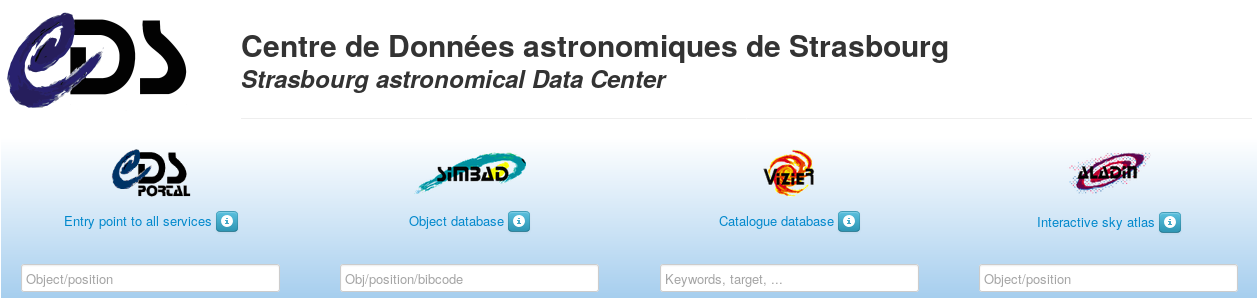
\includegraphics[width=.5\textwidth]{portal-cds}\\
    \hspace{.40\textwidth}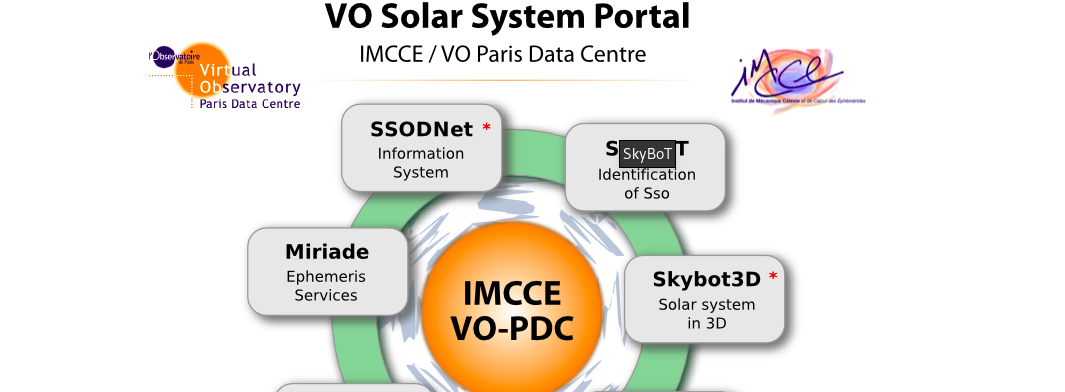
\includegraphics[width=.5\textwidth]{portal-imcce}
  \end{block}
% http://vo.imcce.fr/webservices/miriade/vision_query.php?-name=a:Tama,a:Funke,a:Zero,a:Charlois&-nbd=1&-step=1&-observer=010&-ep=now&-from=Demo&-mime=pdf

\end{frame}
%%%%%%%----  END  ----  ----%%%%%%



\subsection{Visibility of targets}
%%%%%%%---- BEGIN ----  ----%%%%%%
\begin{frame}
  \frametitle{Visibility of targets}

  \begin{exampleblock}{Example}
    Can I observe asteroids Ceres, Pallas, 4321 tonight? And M31?
  \end{exampleblock}

  \begin{block}{Answer: ViSiON}
    \hspace{.25\textwidth}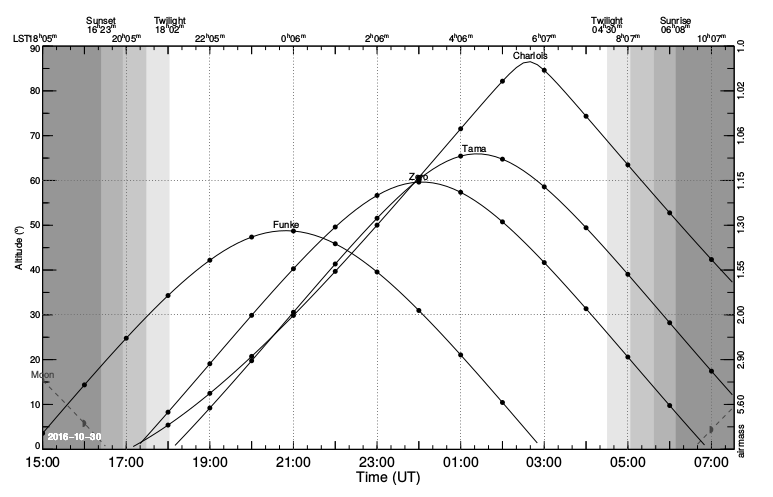
\includegraphics[width=.5\textwidth]{vision}
  \end{block}
% http://vo.imcce.fr/webservices/miriade/vision_query.php?-name=a:Ceres, a:Pallas,a:Zero,u:M_31&-nbd=1&-step=1&-observer=010&-ep=now&-from=Demo&-mime=pdf

\end{frame}
%%%%%%%----  END  ----  ----%%%%%%



\subsection{Accessing data}
%%%%%%%---- BEGIN ----  ----%%%%%%
\begin{frame}
  \frametitle{Accessing data}

  \begin{exampleblock}{Example}
    What is the diameter of Groussin? The taxonomy of Vernazza?
  \end{exampleblock}

  \begin{block}{Answer: ViZieR and Aladin}
    %\hspace{.15\textwidth}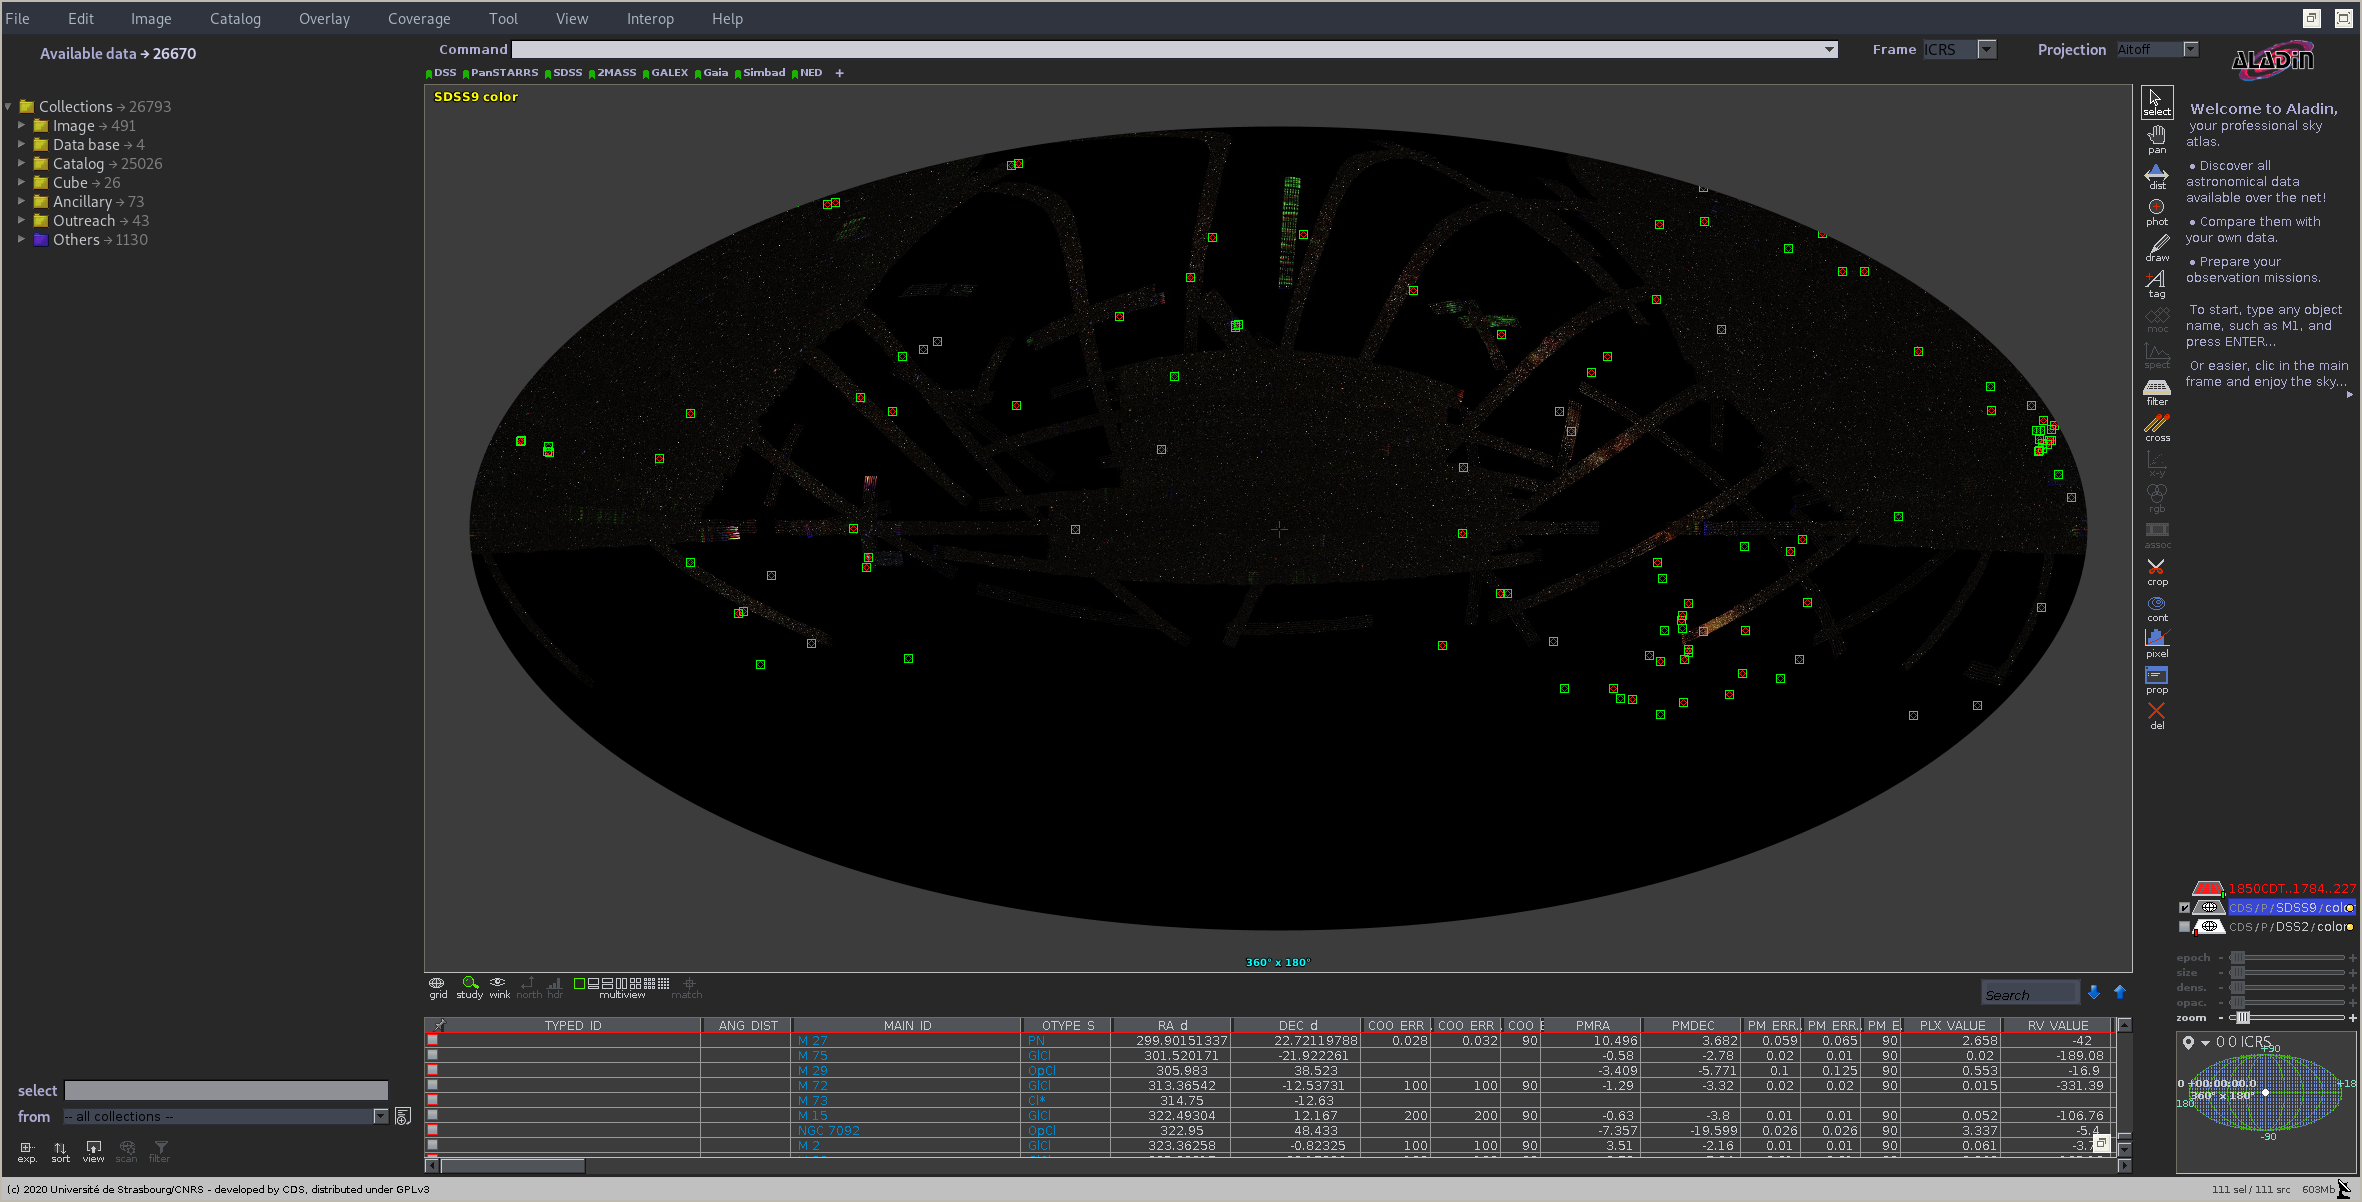
\includegraphics[width=.7\textwidth]{messier_sdss}
  \end{block}
%http://simbad.u-strasbg.fr/simbad/sim-ref?bibcode=1850CDT..1784..227M&simbo=on
\end{frame}
%%%%%%%----  END  ----  ----%%%%%%



